\documentclass{standalone}

%x description="plot marks"
\usepackage{pgfplots}
\pgfplotsset{compat=newest, width=3cm, height=2.5cm}

\begin{document}
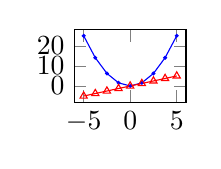
\begin{tikzpicture}
\begin{axis}[mark size=1.5pt, samples=9]
%x step={
	% addplot+ adds options
	\addplot+[mark size=0.5pt] {x^2};
	\addplot+[mark=triangle] {x};
%x }
\end{axis}
\end{tikzpicture}

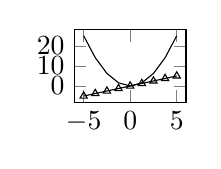
\begin{tikzpicture}
\begin{axis}[mark size=1.5pt, samples=9]
%x step={
	% using only addplot overwrites them
	% mark size alone has no effect, as no mark is defined
	\addplot[mark size=0.5pt] {x^2};
	\addplot[mark=triangle] {x};
%x }
\end{axis}
\end{tikzpicture}

\end{document}
